\documentclass[journal,12pt,twocolumn]{IEEEtran}
\usepackage{setspace}
\usepackage{gensymb}
\usepackage{caption}
%\usepackage{multirow}
%\usepackage{multicolumn}
%\usepackage{subcaption}
%\doublespacing
\singlespacing
\usepackage{csvsimple}
\usepackage{amsmath}
\usepackage{multicol}
%\usepackage{enumerate}
\usepackage{amssymb}
%\usepackage{graphicx}
\usepackage{newfloat}
%\usepackage{syntax}
\usepackage{listings}
\usepackage{color}
\usepackage{tikz}
\usetikzlibrary{shapes,arrows}



%\usepackage{graphicx}
%\usepackage{amssymb}
%\usepackage{relsize}
%\usepackage[cmex10]{amsmath}
%\usepackage{mathtools}
%\usepackage{amsthm}
%\interdisplaylinepenalty=2500
%\savesymbol{iint}
%\usepackage{txfonts}
%\restoresymbol{TXF}{iint}
%\usepackage{wasysym}
\usepackage{amsthm}
\usepackage{mathrsfs}
\usepackage{txfonts}
\usepackage{stfloats}
\usepackage{cite}
\usepackage{cases}
\usepackage{mathtools}
\usepackage{caption}
\usepackage{enumerate}	
\usepackage{enumitem}
\usepackage{amsmath}
%\usepackage{xtab}
\usepackage{longtable}
\usepackage{multirow}
%\usepackage{algorithm}
%\usepackage{algpseudocode}
\usepackage{enumitem}
\usepackage{mathtools}
\usepackage{hyperref}
%\usepackage[framemethod=tikz]{mdframed}
\usepackage{listings}
    %\usepackage[latin1]{inputenc}                                 %%
    \usepackage{color}                                            %%
    \usepackage{array}                                            %%
    \usepackage{longtable}                                        %%
    \usepackage{calc}                                             %%
    \usepackage{multirow}                                         %%
    \usepackage{hhline}                                           %%
    \usepackage{ifthen}                                           %%
  %optionally (for landscape tables embedded in another document): %%
    \usepackage{lscape}     


\usepackage{url}
\def\UrlBreaks{\do\/\do-}


%\usepackage{stmaryrd}


%\usepackage{wasysym}
%\newcounter{MYtempeqncnt}
\DeclareMathOperator*{\Res}{Res}
%\renewcommand{\baselinestretch}{2}
\renewcommand\thesection{\arabic{section}}
\renewcommand\thesubsection{\thesection.\arabic{subsection}}
\renewcommand\thesubsubsection{\thesubsection.\arabic{subsubsection}}

\renewcommand\thesectiondis{\arabic{section}}
\renewcommand\thesubsectiondis{\thesectiondis.\arabic{subsection}}
\renewcommand\thesubsubsectiondis{\thesubsectiondis.\arabic{subsubsection}}
\providecommand{\gauss}[2]{\mathcal{N}\ensuremath{\left(#1,#2\right)}}
% correct bad hyphenation here
\hyphenation{op-tical net-works semi-conduc-tor}

%\lstset{
%language=C,
%frame=single, 
%breaklines=true
%}

%\lstset{
	%%basicstyle=\small\ttfamily\bfseries,
	%%numberstyle=\small\ttfamily,
	%language=Octave,
	%backgroundcolor=\color{white},
	%%frame=single,
	%%keywordstyle=\bfseries,
	%%breaklines=true,
	%%showstringspaces=false,
	%%xleftmargin=-10mm,
	%%aboveskip=-1mm,
	%%belowskip=0mm
%}

%\surroundwithmdframed[width=\columnwidth]{lstlisting}
\def\inputGnumericTable{}                                 %%
\lstset{
%language=C,
frame=single, 
breaklines=true,
columns=fullflexible
}
 

\begin{document}
%
\tikzstyle{block} = [rectangle, draw,
    text width=3em, text centered, minimum height=3em]
\tikzstyle{sum} = [draw, circle, node distance=3cm]
\tikzstyle{input} = [coordinate]
\tikzstyle{output} = [coordinate]
\tikzstyle{pinstyle} = [pin edge={to-,thin,black}]

\theoremstyle{definition}
\newtheorem{theorem}{Theorem}[section]
\newtheorem{problem}{Problem}
\newtheorem{proposition}{Proposition}[section]
\newtheorem{lemma}{Lemma}[section]
\newtheorem{corollary}[theorem]{Corollary}
\newtheorem{example}{Example}[section]
\newtheorem{definition}{Definition}[section]
%\newtheorem{algorithm}{Algorithm}[section]
%\newtheorem{cor}{Corollary}
\newcommand{\BEQA}{\begin{eqnarray}}
\newcommand{\EEQA}{\end{eqnarray}}
\newcommand{\define}{\stackrel{\triangle}{=}}

\bibliographystyle{IEEEtran}
%\bibliographystyle{ieeetr}

\providecommand{\nCr}[2]{\,^{#1}C_{#2}} % nCr
\providecommand{\nPr}[2]{\,^{#1}P_{#2}} % nPr
\providecommand{\mbf}{\mathbf}
\providecommand{\pr}[1]{\ensuremath{\Pr\left(#1\right)}}
\providecommand{\qfunc}[1]{\ensuremath{Q\left(#1\right)}}
\providecommand{\sbrak}[1]{\ensuremath{{}\left[#1\right]}}
\providecommand{\lsbrak}[1]{\ensuremath{{}\left[#1\right.}}
\providecommand{\rsbrak}[1]{\ensuremath{{}\left.#1\right]}}
\providecommand{\brak}[1]{\ensuremath{\left(#1\right)}}
\providecommand{\lbrak}[1]{\ensuremath{\left(#1\right.}}
\providecommand{\rbrak}[1]{\ensuremath{\left.#1\right)}}
\providecommand{\cbrak}[1]{\ensuremath{\left\{#1\right\}}}
\providecommand{\lcbrak}[1]{\ensuremath{\left\{#1\right.}}
\providecommand{\rcbrak}[1]{\ensuremath{\left.#1\right\}}}
\theoremstyle{remark}
\newtheorem{rem}{Remark}
\newcommand{\sgn}{\mathop{\mathrm{sgn}}}
% \providecommand{\abs}[1]{\left\vert#1\right\vert}
\providecommand{\res}[1]{\Res\displaylimits_{#1}} 
% \providecommand{\norm}[1]{\left\Vert#1\right\Vert}
\providecommand{\mtx}[1]{\mathbf{#1}}
% \providecommand{\mean}[1]{E\left[ #1 \right]}
\providecommand{\fourier}{\overset{\mathcal{F}}{ \rightleftharpoons}}
%\providecommand{\hilbert}{\overset{\mathcal{H}}{ \rightleftharpoons}}
\providecommand{\system}{\overset{\mathcal{H}}{ \longleftrightarrow}}
	%\newcommand{\solution}[2]{\textbf{Solution:}{#1}}
\newcommand{\solution}{\noindent \textbf{Solution: }}
\newcommand{\myvec}[1]{\ensuremath{\begin{pmatrix}#1\end{pmatrix}}}
\providecommand{\dec}[2]{\ensuremath{\overset{#1}{\underset{#2}{\gtrless}}}}
\DeclarePairedDelimiter{\ceil}{\lceil}{\rceil}
%\numberwithin{equation}{section}
%\numberwithin{problem}{subsection}
%\numberwithin{definition}{subsection}
\makeatletter
\@addtoreset{figure}{section}
\makeatother

\let\StandardTheFigure\thefigure
%\renewcommand{\thefigure}{\theproblem.\arabic{figure}}
\renewcommand{\thefigure}{\thesection}


%\numberwithin{figure}{subsection}

%\numberwithin{equation}{subsection}
%\numberwithin{equation}{section}
%\numberwithin{equation}{problem}
%\numberwithin{problem}{subsection}
\numberwithin{problem}{section}
%%\numberwithin{definition}{subsection}
%\makeatletter
%\@addtoreset{figure}{problem}
%\makeatother

\makeatletter
\@addtoreset{table}{section}
\makeatother

\let\StandardTheFigure\thefigure
\let\StandardTheTable\thetable
\let\vec\mathbf
\numberwithin{equation}{section}

\vspace{3cm}


\title{%Convex Optimization in Python
	Random Numbers
}
%\title{
%	\logo{Matrix Analysis through Octave}{\begin{center}\includegraphics[scale=.24]{tlc}\end{center}}{}{HAMDSP}
%}


% paper title
% can use linebreaks \\ within to get better formatting as desired
%\title{Matrix Analysis through Octave}
%
%
% author names and IEEE memberships
% note positions of commas and nonbreaking spaces ( ~ ) LaTeX will not break
% a structure at a ~ so this keeps an author's name from being broken across
% two lines.
% use \thanks{} to gain access to the first footnote area
% a separate \thanks must be used for each paragraph as LaTeX2e's \thanks
% was not built to handle multiple paragraphs
%

\author{Nitya Seshagiri Bhamidipaty - CS21BTECH11041}
% note the % following the last \IEEEmembership and also \thanks - 
% these prevent an unwanted space from occurring between the last author name
% and the end of the author line. i.e., if you had this:
% 
% \author{....lastname \thanks{...} \thanks{...} }
%                     ^------------^------------^----Do not want these spaces!
%
% a space would be appended to the last name and could cause every name on that
% line to be shifted left slightly. This is one of those "LaTeX things". For
% instance, "\textbf{A} \textbf{B}" will typeset as "A B" not "AB". To get
% "AB" then you have to do: "\textbf{A}\textbf{B}"
% \thanks is no different in this regard, so shield the last } of each \thanks
% that ends a line with a % and do not let a space in before the next \thanks.
% Spaces after \IEEEmembership other than the last one are OK (and needed) as
% you are supposed to have spaces between the names. For what it is worth,
% this is a minor point as most people would not even notice if the said evil
% space somehow managed to creep in.



% The paper headers
%\markboth{Journal of \LaTeX\ Class Files,~Vol.~6, No.~1, January~2007}%
%{Shell \MakeLowercase{\textit{et al.}}: Bare Demo of IEEEtran.cls for Journals}
% The only time the second header will appear is for the odd numbered pages
% after the title page when using the twoside option.
% 
% *** Note that you probably will NOT want to include the author's ***
% *** name in the headers of peer review papers.                   ***
% You can use \ifCLASSOPTIONpeerreview for conditional compilation here if
% you desire.




% If you want to put a publisher's ID mark on the page you can do it like
% this:
%\IEEEpubid{0000--0000/00\$00.00~\copyright~2007 IEEE}
% Remember, if you use this you must call \IEEEpubidadjcol in the second
% column for its text to clear the IEEEpubid mark.



% make the title area
\maketitle

\tableofcontents
% \bigskip


% 
% \renewcommand{\thefigure}{\theenumi}
% \renewcommand{\thetable}{\theenumi}

% \begin{abstract}
%     This manual provides a simple introduction to the generation of random numbers
%     \end{abstract}

\section{Uniform Random Numbers}
Let $U$ be a uniform random variable between 0 and 1.
\begin{enumerate}[label=\thesection.\arabic*
,ref=\thesection.\theenumi]
\item Generate $10^6$ samples of $U$ using a C program and save into a file called uni.dat .
\\
\solution
\begin{lstlisting}
 wget https://github.com/NityaBhamidipaty/RandAssig/blob/main/codes/coeffs.h
  
 wget https://github.com/NityaBhamidipaty/RandAssig/blob/main/codes/main.c
\end{lstlisting}
\item
Load the uni.dat file into python and plot the empirical CDF of $U$ using the samples in uni.dat. The CDF is defined as
\begin{align}
F_{U}(x) = \pr{U \le x}
\end{align}
\\
\solution
The fig \ref{fig:uni_cdf} is plotted using the code:
\begin{lstlisting}
wget https://github.com/NityaBhamidipaty/RandAssig/blob/main/codes/cdf_plot.py
\end{lstlisting}
\begin{figure}[h]
    \centering
    \includegraphics[width=\columnwidth]{figs/uni_cdf.pdf}
    \caption{CDF of U}
    \label{fig:uni_cdf}
\end{figure}
\item
Find a  theoretical expression for $F_{U}(x)$.
\\
\solution
\begin{align}
    f_U(x) &= \begin{cases}
    1 & x\in(0,1)\\
    0 & \text{otherwise}
    \end{cases}\\
    F_U(x) &= \int_{-\infty}^{x}f_U(u)dx\\
\end{align}
if $x \le 0$
\begin{align}
    F_U(x) &= \int_{-\infty}^{x}f_U(u)dx\\
        &= \int_{-\infty}^{x}0dx\\
        &= 0
\end{align}
if $x \in (0,1)$
\begin{align}
    F_U(x) &= \int_{-\infty}^{x}f_U(u)dx\\
        &= \int_{-\infty}^{x}1dx\\
        &= x
\end{align}
if $x \ge 1$
\begin{align}
    F_U(x) &= \int_{-\infty}^{x}f_U(u)dx\\
        &= \int_{-\infty}^{x}0dx\\
        &= 0
\end{align}
Hence,
\begin{align}
    F_U(x) &= \begin{cases}
     0 & x\le0\\
     x & x\in(0,1)\\
     1 & x\ge1
    \end{cases}
\end{align}
\item
The mean of $U$ is defined as
%
\begin{equation}
E\sbrak{U} = \frac{1}{N}\sum_{i=1}^{N}U_i
\end{equation}
%
and its variance as
%
\begin{equation}
\text{var}\sbrak{U} = E\sbrak{U- E\sbrak{U}}^2 
\end{equation}

Write a C program to  find the mean and variance of $U$. 
\\
\solution
\begin{align}
    E[X] &= 0.500007\\
    Var[X] &= 0.083301
\end{align}
\begin{lstlisting}
wget https://github.com/NityaBhamidipaty/RandAssig/blob/main/codes/coeffs.h  
wget https://github.com/NityaBhamidipaty/RandAssig/blob/main/codes/main.c
\end{lstlisting}

\item Verify your result theoretically given that

\begin{equation}
E\sbrak{U^k} = \int_{-\infty}^{\infty}x^kdF_{U}(x)
\end{equation}
\solution
\begin{align}
    E[U^k] &= \int_{-\infty}^{\infty} x^k dF_U(x)\\
            &= \int_{-\infty}^{0} 0 + \int_{0}^{1}x^kdx + \int_1^{\infty}0\\
            &= \frac{1}{k+1}\\
    \implies E[U] &= \frac{1}{2}
\end{align}
%
\end{enumerate}

\section{Central Limit Theorem}
%
\begin{enumerate}[label=\thesection.\arabic*
,ref=\thesection.\theenumi]

%
\item
Generate $10^6$ samples of the random variable
%
\begin{equation}
X = \sum_{i=1}^{12}U_i -6
\end{equation}
%
using a C program, where $U_i, i = 1,2,\dots, 12$ are  a set of independent uniform random variables between 0 and 1
and save in a file called gau.dat
\\
\solution
\begin{lstlisting}
wget https://github.com/NityaBhamidipaty/RandAssig/blob/main/codes/coeffs.h
wget https://github.com/NityaBhamidipaty/RandAssig/blob/main/codes/main.c
\end{lstlisting}
\item
Load gau.dat in python and plot the empirical CDF of $X$ using the samples in gau.dat. What properties does a CDF have?
\\
\solution
The fig\ref{fig:gau_cdf} is plotted using:
\begin{lstlisting}
wget https://github.com/NityaBhamidipaty/RandAssig/blob/main/codes/cdf_plot.py
\end{lstlisting}
\begin{figure}[h]
    \centering
    \includegraphics[width=\columnwidth]{./figs/gau_cdf.pdf}
    \caption{CDF of X}
    \label{fig:gau_cdf}
\end{figure}
Properties of CDF
\begin{enumerate}
    \item $x\rightarrow{-\infty}\text{        } F_U(x) \rightarrow{0}$
    \item $x\rightarrow{\infty}\text{        } F_U(x) \rightarrow{1}$
    \item $F_U(x)$ is non-decreasing.
    \item $F_U(x)$ is non-negative.
\end{enumerate}
\item
Load gau.dat in python and plot the empirical PDF of $X$ using the samples in gau.dat. The PDF of $X$ is defined as
\begin{align}
p_{X}(x) = \frac{d}{dx}F_{X}(x)
\end{align}
What properties does the PDF have?
\\
\solution The PDF of $X$ (\ref{fig:gau_pdf})is plotted using the code below:
\begin{lstlisting}
wget https://github.com/NityaBhamidipaty/RandAssig/blob/main/codes/pdf_plot.py
\end{lstlisting}
\begin{figure}[h]
    \centering
    \includegraphics[width=\columnwidth]{./figs/gauss_pdf.pdf}
    \caption{PDF of $X$}
    \label{fig:gau_pdf}
\end{figure}
Properties of PDF
\begin{enumerate}
    \item $x\rightarrow{-\infty}\text{        } f_U(x) \rightarrow{0}$
    \item $x\rightarrow{\infty}\text{        } f_U(x) \rightarrow{0}$
    \item $f_U(x)$ is non-negative.
\end{enumerate}
\item Find the mean and variance of $X$ by writing a C program.\\
\solution
\begin{align}
    E[X] &= 0.000326\\
Var[X] &= 1.000906
\end{align}
\begin{lstlisting}
wget https://github.com/NityaBhamidipaty/RandAssig/blob/main/codes/coeffs.h
wget https://github.com/NityaBhamidipaty/RandAssig/blob/main/codes/main.c
\end{lstlisting}
\item Given that 
\begin{align}
p_{X}(x) = \frac{1}{\sqrt{2\pi}}\exp\brak{-\frac{x^2}{2}}, -\infty < x < \infty,
\end{align}
repeat the above exercise theoretically.\\
\solution
\begin{align}
    E(X) &= \int_{-\infty}^{\infty}\frac{1}{\sqrt{2\pi}}\exp\brak{-\frac{x^2}{2}}x\,dx
    %  &= \int_{\infty}^{\infty}\frac{1}{\sqrt{2\pi}}\exp\brak{-u}\,du\\
     = 0 \\
     & \text{Since the integrand is odd}
\end{align}

\begin{align}
    Var(X) &=\int_{-\infty}^{\infty}x^2\frac{1}{\sqrt{2\pi}}\exp\brak{-\frac{x^2}{2}}\,dx\\
    &= \int_{-\infty}^{\infty}\frac{1}{\sqrt{2\pi}}x(xe^{-\frac{x^2}{2}})\,dx\\
    &= -\frac{1}{\sqrt{2\pi}}xe^{-\frac{x^2}{2}}|_{-\infty}^{\infty} + \int_{-\infty}^{\infty}\frac{1}{\sqrt{2\pi}}e^{-\frac{x^2}{2}}\,dx
    % -\frac{1}{\sqrt{2\pi}}xe^{-\frac{x^2}{2}}|_{-\infty}^{\infty} &= \lim-\frac{1}{\sqrt{2\pi}}xe^{-\frac{x^2}{2}}|_{-r}^{r}
\end{align}
\begin{align}
        -\frac{1}{\sqrt{2\pi}}xe^{-\frac{x^2}{2}}|_{-\infty}^{\infty} &= \lim_{x\to\infty}-\frac{1}{\sqrt{2\pi}}xe^{-\frac{x^2}{2}}|_{-r}^{r}\\
        &= \lim_{x\to\infty}-\frac{1}{\sqrt{2\pi}}2\frac{r}{e^{\frac{r^2}{2}}}\\
                &= \lim_{x\to\infty}-\frac{1}{\sqrt{2\pi}}2\frac{1}{re^{\frac{r^2}{2}}}\\
                &= 0
\end{align}
\begin{align}
    \int_{-\infty}^{\infty}\frac{1}{\sqrt{2\pi}}e^{-\frac{x^2}{2}}\,dx &= \frac{1}{\sqrt{\pi}}\int_{-\infty}^{\infty}e^{-\frac{x^2}{2}}\,d\frac{x}{\sqrt{2}}\\
    &= \int_{-\infty}^{\infty}\frac{1}{\sqrt{\pi}}e^{-t^2}\,dt\\
    &= \frac{\sqrt{\pi}}{\sqrt{\pi}} = 1
\end{align}
\end{enumerate}
\section{From Uniform to Other}
\begin{enumerate}[label=\thesection.\arabic*
,ref=\thesection.\theenumi]
%
\item
Generate samples of 
%
\begin{equation}
V = -2\ln\brak{1-U}
\end{equation}
%
and plot its CDF.  \\
\solution
The CDF of $V$ (\ref{fig:other_cdf}) is plotted using the code below:
\begin{lstlisting}
wget https://github.com/NityaBhamidipaty/RandAssig/blob/main/codes/cdf_plot.py
\end{lstlisting}
\begin{figure}
    \centering
    \includegraphics[width=\columnwidth]{./figs/other_cdf.pdf}
    \caption{CDF of $V$}
    \label{fig:other_cdf}
\end{figure}
\item Find a theoretical expression for $F_V(x)$.\\
\solution
\begin{align}
    V &= -2\ln(1-U)\\
    F_V(x) &= P\{V\le x\}\\
    &= P\{-2\ln(1-U)\le x\}\\
    &= P\{U\le1-e^{-\frac{x}{2}}\}\\
    &= F_U(1-e^{-\frac{x}{2}})
\end{align}
Case 1
\begin{align}
    F_V(x) &= F_U(1-e^{-\frac{x}{2}}) = 0\\
    1-e^{-\frac{x}{2}} &\le 0\\
    1 &\le e^{-\frac{x}{2}}\\
    0 &\le -\frac{x}{2}\\
    x &\le 0
\end{align}
Case 2
\begin{align}
    F_V(x) &= F_U(1-e^{-\frac{x}{2}}) = 1-e^{-\frac{x}{2}}\\
    0 &< 1-e^{-\frac{x}{2}} < 1 \\
\end{align}
$1-e^{-\frac{x}{2}} < 1$ is always true as $e^{-\frac{x}{2}} > 0$
\begin{align}
    0 &< 1-e^{-\frac{x}{2}}\\
    -1 &< -e^{-\frac{x}{2}}\\
    1 &> e^{-\frac{x}{2}}\\
    0 &> -\frac{x}{2}\\
    0 &< x
\end{align}
Case 3
\begin{align}
    1-e^{-\frac{x}{2}} &\ge 1\\
    0 &\ge e^{-\frac{x}{2}}\\
    x \in \phi
\end{align}
Hence,
\begin{align}
    F_V(x) &= \begin{cases}
                0 & x\le0\\
                1 - e^{-\frac{x}{2}} & x>0
    \end{cases}
\end{align}
\end{enumerate}
\section{Triangular Distribution}

\begin{enumerate}[label=\thesection.\arabic*
    ,ref=\thesection.\theenumi]
\item Generate 
\begin{align}
    T &= U_1 + U_2
\end{align}
\solution
\begin{lstlisting}
wget https://github.com/NityaBhamidipaty/RandAssig/blob/main/codes/main.c
\end{lstlisting}
\item Find the CDF of T\\
\solution\\
The CDF (\ref{fig:cdf_T}) is plotted using 
\begin{lstlisting}
wget https://github.com/NityaBhamidipaty/RandAssig/blob/main/codes/cdf_plot.py
\end{lstlisting}
\begin{figure}
    \centering
    \includegraphics[width=\columnwidth]{./figs/tri_cdf.pdf}
    \caption{CDF of T}
    \label{fig:cdf_T}
\end{figure}
\item Find the PDF of T\\
\solution
The PDF (\ref{fig:pdf_T}) is plotted using
\begin{lstlisting}
weget https://github.com/NityaBhamidipaty/RandAssig/blob/main/codes/pdf_plot.py
\end{lstlisting}
\begin{figure}
    \centering
    \includegraphics[width=\columnwidth]{./figs/tri_pdf.pdf}
    \caption{PDF of $T$}
    \label{fig:pdf_T}
\end{figure}
\item Find the theoretical expressions of CDF an PDF of T.\\
\solution
\begin{align}
    f_T(t) &= \int_{-\infty}^{\infty}f_{U_2}(x)f_{U_1}(t-x)\,dx\\
    &= \int_{0}^{1}f(x)f(t-x)\,dx
\end{align}
If $t\in(0,1)$
\begin{align}
    f_T(t) &= \int_{0}^{t}1\times1\,dx\\
    &= t
\end{align}
If $t\in(1,2)$
\begin{align}
    f_T(t) &= \int_{t-1}^{1}1\times1\,dx\\
    &= 2 -t
\end{align}
Hence,
\begin{align}
    f_T(t) &= \begin{cases}
    t & t\in(0,1)\\
    2-t & t\in(1,2)\\
    0 & \text{otherwise}
    \end{cases}
\end{align}
\begin{align}
    F_T(t) &= \int_{-\infty}^{t}f_T(t)\,dt\\
    \end{align}
    \begin{align}
    F_T(t) &= \begin{cases}
    0 & t\le0\\
    \frac{t^2}{2} & t\in(0,1)\\
    \frac{-t^2}{2} +2t -1 & t\in(1,2)\\
    1         & t\ge2
    \end{cases}
\end{align}
\end{enumerate}
\section{Maximum Likelihood}
\begin{enumerate}[label=\thesection.\arabic*
    ,ref=\thesection.\theenumi]
\item Generate equiprobable $X \in \{1, -1\}$\\
\solution
\begin{lstlisting}
weget ...
\end{lstlisting}
\item Generate 
\begin{align}
    Y &= AX + N
\end{align}
where $A = 5$ dB and $N \sim \mathcal{N}(0,1)$\\
\solution\\
\begin{lstlisting}
weget ...
\end{lstlisting}
\item Plot $Y$ using scatter plot\\
\solution\\
The plot \ref*{fig:scatter_y} is plotted using
\begin{lstlisting}
    weget ...
\end{lstlisting}
\begin{figure}
    \centering
    \includegraphics[width=\columnwidth]{./figs/scatter.png}
    \label{fig:scatter_y}
\end{figure}
\item Guess how to estimate $X$ from $Y$\\
\solution\\
Estimated value of $X = \hat{X}$

\begin{align}
   \hat{X} &= \begin{cases} -1 & Y<0\\ 1 & Y\ge \end{cases}
\end{align} 


\item Find 
\begin{equation}
	P_{e|0} = \pr{\hat{X} = -1|X=1}
\end{equation}
and 
\begin{equation}
	P_{e|1} = \pr{\hat{X} = 1|X=-1}
\end{equation}
\solution
\begin{align}
	P_{e|0} &= \pr{\hat{X} = -1|X=1} = 0.49999\\
	P_{e|1} &= \pr{\hat{X} = 1|X=-1} = 0.50075
\end{align}
\begin{lstlisting}
    weget ...
\end{lstlisting}
\item  Find $P_e$ assuming that $X$ has equiprobable symbols.\\
\solution
\begin{align}
    P_e &= P(X=1)P_{e|0} + P(X = -1)P_{e|1}\\
    &= \frac{1}{2}(P_{e|0} + P_{e|1})\\
    &= \frac{1}{2}(0.49999+0.50075)\\
    &= 0.50037
\end{align}
\item Verify by plotting  the theoretical $P_e$ with respect to $A$ from 0 to 10 dB.  \\
\solution
\begin{align}
    P_e &= P_{e|0}P(X = 1) + P_{e|1}P(X=-1)\\
    &= \frac{1}{2}(P_{e|0}+P_{e|1})
\end{align}
\begin{align}
    P_{e|0} &= P(Y\le0|X=1)\\
    &= P(AX+N \le 0|X=1)\\
    &= P(A+N\le0)\\
    &= P(N\le-A)\\
    &= P(N>A) 
\end{align}
\begin{align}
    P_{e|1} &= P(Y>0|X=-1)\\
    &= P(AX+N > 0|X=-1)\\
    &= P(-A+N>0)\\
    &= P(N>A)
\end{align}
\begin{align}
    P_e &= P(N>A)=Q(A) 
\end{align}
Plotted using code
\begin{lstlisting}
    weget ...
\end{lstlisting}
\begin{figure}
    \centering
    \includegraphics[width=\columnwidth]{./figs/pevsa.pdf}
    \caption{$P_e(A)$ vs $A$}
    \label{fig:pevsa}
\end{figure}
\item Now, consider a threshold $\delta$  while estimating $X$ from $Y$. Find the value of $\delta$ that maximizes the theoretical $P_e$.\\
\solution\\
\begin{align}
    \hat{X} &= \begin{cases} 1 & Y>\delta\\
        -1 & Y<\delta
    \end{cases}
\end{align}
\begin{align}
    P_{e|0} &= P(Y < \delta | X = 1)\\
    &= P(AX+N < \delta|X=1)\\
    &= P(A+N < \delta)\\
    &= P(N < \delta - A)\\
    &= P(N >  A - \delta)\\
    &= Q(A-\delta)
\end{align}
\begin{align}
    P_{e|1} &= P(Y > \delta | X = -1)\\
    &= P(-A+N > \delta|X=-1)\\
    &= P(-A+N > \delta)\\
    &= P(N > \delta + A)\\
    &= Q(A+\delta)
\end{align}
\begin{align}
    P_e &= \frac{1}{2}(Q(A+\delta)+Q(A-\delta))
\end{align}
Differentiating wrt $\delta$ to find maximum
\begin{equation}
    \frac{d Q(x)}{d x} &= -\frac{1}{\sqrt{2\pi}}e^{\frac{-x^2}{2}}
\end{equation}
\begin{align}
    \frac{d P_e}{d\delta} &= \frac{1}{2}(\frac{1}{\sqrt{2\pi}}e^{-\frac{(A-\delta)^2}{2}} - \frac{1}{\sqrt{2\pi}}e^{-\frac{(A+\delta)^2}{2}})\\
    &= 0\\
    \implies \delta = 0 \text{ or }\\
    A = 0 , \delta\in\mathbb{R}
\end{align}
Verifying it is maximum 
\item Repeat the above exercise when 
\begin{align}
    p_{X}(0) = p
\end{align}
\solution\\
\begin{align}
    P_e &= (1-p)Q(A+\delta)+Q(A-\delta)p
\end{align}
Differentiating
\begin{align}
    \frac{d P_e}{d\delta} &= p\frac{1}{\sqrt{2\pi}}e^{-\frac{(A-\delta)^2}{2}} - \frac{1}{\sqrt{2\pi}}e^{-\frac{(A+\delta)^2}{2}}(1-p)\\
    &= 0\\
\end{align}
\begin{align}
    pe^{-\frac{(\delta-A)^2}{2}} &= (1-p)e^{-\frac{(A+\delta)^2}{2}}\\
    \implies \delta = \frac{1}{2A}\ln\brak{\frac{1-p}{p}}
\end{align}
\item Repeat the above exercise using the MAP criterion.\\
\solution
\begin{align}
    P(X = 1|Y = y) &= \frac{P(Y = y, X = 1)P(X =1)}{P(Y=y)}\\
    &= \frac{P(A+N=y)p}{f_Y(y)}\\
    &= \frac{f_N(y-A)p}{f_Y(y)}
\end{align}
\begin{align}
    P(X = -1|Y = y) &= \frac{P(Y = y, X = -1)P(X =-1)}{P(Y=y)}\\
    &= \frac{P(-A+N=y)(1-p)}{f_Y(y)}\\
    &= \frac{f_N(y+A)(1-p)}{f_Y(y)}
\end{align}
For max error
\begin{align}
    \frac{f_N(y+A)(1-p)}{f_Y(y)} &=  \frac{f_N(y-A)p}{f_Y(y)}\\
    e^{-Ay}(1-p) &=  e^{Ay}p\\
    \implies y &= \frac{1}{2A}\ln\brak{\frac{1-p}{p}} 
\end{align}
\end{enumerate}
\section{Gaussian to Other}
\begin{enumerate}[label=\thesection.\arabic*
    ,ref=\thesection.\theenumi]
\item
Let $X_1 \sim  \gauss{0}{1}$ and $X_2 \sim  \gauss{0}{1}$. Plot the CDF and PDF of
%
\begin{equation}
V = X_1^2 + X_2^2
\end{equation}
\solution
The code for plotting the cdf and pdf
\begin{lstlisting}
    weget ...
\end{lstlisting}
\begin{figure}
    \centering
    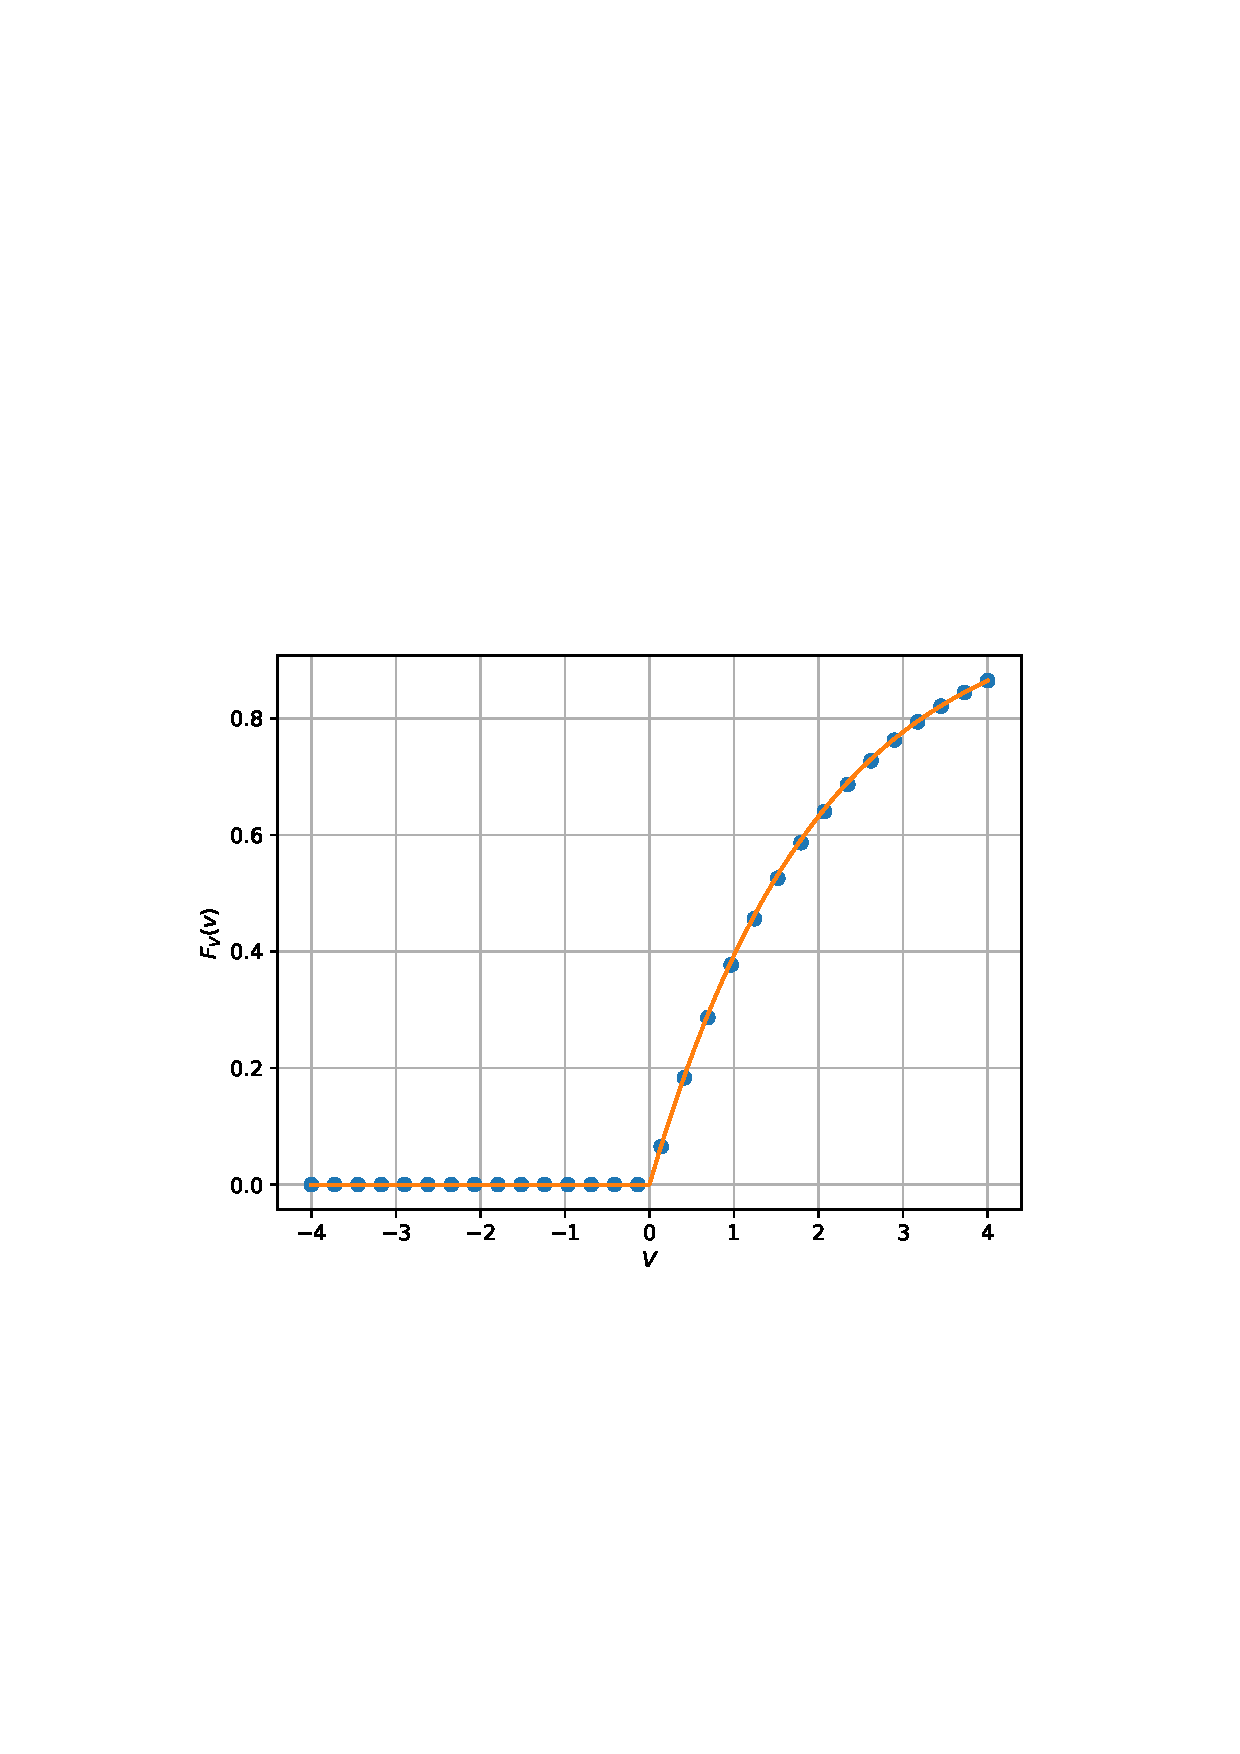
\includegraphics[width=\columnwidth]{./figs/squgau_cdf.pdf}
    \label{fig:vcdf}
\end{figure}
\begin{figure}
    \centering
    \includegraphics[width=\columnwidth]{./figs/squgau_pdf.pdf}
    \label{fig:vpdf}
\end{figure}
\item
If
%
\begin{equation}
F_{V}(x) = 
\begin{cases}
1 - e^{-\alpha x} & x \geq 0 \\
0 & x < 0,
\end{cases}
\end{equation}
%
find $\alpha$.
%
\item
Plot the CDF and PDf of
\begin{equation}
A = \sqrt{V}
\end{equation}
\solution
The code to plot the cdf and pdf
\begin{lstlisting}
    weget ... 
\end{lstlisting}
\begin{figure}
    \centering
    \includegraphics[width=\columnwidth]{./figs/sqrsqugau_cdf.pdf}
    \label{fig:apdf}
\end{figure}
\begin{figure}
    \centering
    \includegraphics[width=\columnwidth]{./figs/sqrsqugau_pdf.pdf}
    \label{fig:apdf}
\end{figure}
\end{enumerate}
\end{enumerate}
\end{document}
